\documentclass{article}

\makeatletter
\renewcommand{\fnum@figure}{Εικόνα \thefigure}
\makeatother

\usepackage[greek, english]{babel}
\usepackage{alphabeta}
\usepackage{atbegshi, picture}

% Set page size and margins
% Replace `letterpaper' with`a4paper' for UK/EU standard size
\usepackage[letterpaper,top=2cm,bottom=2cm,left=3cm,right=3cm,marginparwidth=1.75cm]{geometry}

% Useful packages
\usepackage{amsmath}
\usepackage{graphicx}
\usepackage[colorlinks=true, allcolors=blue]{hyperref}
\usepackage[utf8]{inputenc}
\usepackage{indentfirst}

\newcommand\T{\rule{0pt}{2.6ex}}       % Top strut
\newcommand\B{\rule[-1.2ex]{0pt}{0pt}} 


\addto\captionsenglish{
  \renewcommand{\contentsname}
    {Περιεχόμενα}
}

% \title{Feasibility Study}
% \date{}

\begin{document}
% \maketitle

\begin{titlepage}
   \begin{center}
       \vspace*{1cm}

       \textbf{\huge Use Cases}

       \vspace{0.5cm}
        Τεχνολογία Λογισμικού
            
       \vspace{1cm}

       \textbf{Κατερίνα Μητροπούλου\\Στεφανίδης Μάριος\\Αγγελική Κούρου\\Δημήτρης Βεργίνης\\Δημήτρης Βλαχογιάννης}
       
       \begin{figure}[!htb]
        \centering
        
\includegraphics[width=0.5\textwidth]{logo.png}
        \end{figure}
        
        \vspace{0.5cm}
        
        \begin{figure}[!htb]
        \centering
        \includegraphics[width=0.5\textwidth]{UoP.jpg}
        \end{figure}


       \vfill
            
       Τεχνικό Κείμενο για την Τεχνολογία Λογισμικού\\
            
       \vspace{0.5cm}
            
       CEID, ECE\\
       University of Patras\\
            
   \end{center}
\end{titlepage}


 \noindent Η ομάδα μας

\begin{enumerate}
  \item Βεργίνης Δημήτριος, ΑΜ: 1066634 , ECE
  \item Βλαχογιάννης Δημήτριος, ΑΜ: 1067371, CEID
  \item Κούρου Αγγελική, ΑΜ: 1067499 , CEID
  \item Μητροπούλου Αικατερίνα - Quality Manager, ΑΜ: 1067409, CEID
  \item Στεφανίδης Μάριος - Project Manager, ΑΜ:1067458, CEID
\end{enumerate}

{
  \hypersetup{linkcolor=black}
  \tableofcontents
}

\newpage

\section{Εισαγωγή}

Τα Use Cases αποτελούν ένα σύνολο δραστηριοτήτων ή βημάτων που λαμβάνουν χώρα κατά την πλοήγηση ενός χρήστη (ή ρόλου, γνωστού στην UML ως ηθοποιού) σε ένα σύστημα, για να επιτευχθεί ένας στόχος. Ο ηθοποιός μπορεί να είναι άνθρωπος ή κάποιο άλλο εξωτερικό σύστημα. 
Για την ανάπτυξη ενός use case χρησιμοποιούνται τα διαγράμματα περιπτώσεων χρήσης, καθώς και λεκτική περιγραφή των περιπτώσεων αυτών.

\section{Διάγραμμα Περιπτώσεων Χρήσης}

Παρακάτω παρουσιάζεται το διάγραμμα περιπτώσεων χρήσης. Για την καλύτερη κατανόηση του διαγράμματος σημειώνεται ότι:

\begin{enumerate}
  \item Τα σκίτσα με τους ανθρώπους αντιστοιχούν στους ηθοποιούς του εκάστοτε use case, δηλαδή τους εμπλεκόμενους
  \item Οι μπλε ελλείψεις αντιστοιχούν στα use cases
  \item Οι μαύρες γραμμές απεικονίζουν άμεση συσχέτιση μεταξύ ενός ηθοποιού και μίας περίπτωσης χρήσης
  \item Οι μπλε διακεκομμένες γραμμές (το μπλε επιλέχθηκε για ευαναγνωσία) απεικονίζουν τη σχέση εξάρτησης μεταξύ δύο περιπτώσεων χρήσης, δηλαδή το use case στο οποίο δείχνει το βέλος δεν μπορεί να υπάρξει αν δεν έχει προηγηθεί το use case από το οποίο ξεκινάει το βέλος 
\end{enumerate}

\vspace{0.3cm}

\scalebox{1.3}{\textbf{Παρατηρήσεις}}

\vspace{0.2cm}

\par\underline{Παρατήρηση Πρώτη:} Στο παρακάτω διάγραμμα:
\begin{enumerate}
    \item ενώ το use case που αφορά στην διαδικασία log in, είναι προαπαιτούμενο για την ύπαρξη όλων των υπολοίπων, δεν παριστάνονται οι συγκεκριμένες συσχετίσεις εξάρτησης για την καλύτερη παρουσίαση και ευαναγνωσία του διαγράμματος
    \item ενώ το use case που αφορά στην διαδικασία δημιουργίας νέου υπαλλήλου (Creates New Employee), είναι προαπαιτούμενο για την ύπαρξη όλων των υπολοίπων, δεν παριστάνονται οι συγκεκριμένες συσχετίσεις εξάρτησης για την καλύτερη παρουσίαση και ευαναγνωσία του διαγράμματος
\end{enumerate}

\vspace{0.3cm}

\underline{Παρατήρηση Δεύτερη:} Η πρώτη σημείωση ισχύει και παρακάτω στην ανάλυση των περιπτώσεων χρήσης. \par \vspace{0.1cm} Δηλαδή, ενώ τα συγκεκριμένα use cases είναι απαραίτητα προαπαιρούμενα για οποιαδήποτε διεργασία \par πραγματοποιείται εντός του \textbf{Medic World}, δεν αναγράφονται ως προαπαιτούμενα για αποφυγή της \par διαρκούς επανάληψης.  

\vspace{0.3cm}

\underline{Παρατήρηση Τρίτη:} Κάθε μέλος της ομάδας ανέλαβε από δύο use cases και την οργάνωση και τη \par \vspace{0.1cm} σύνταξη της αναφοράς ανέλαβαν οι Μητροπούλου Αικατερίνα και Στεφανίδης Μάριος.  

\newpage

\begin{figure}[!htb]
        \centering
        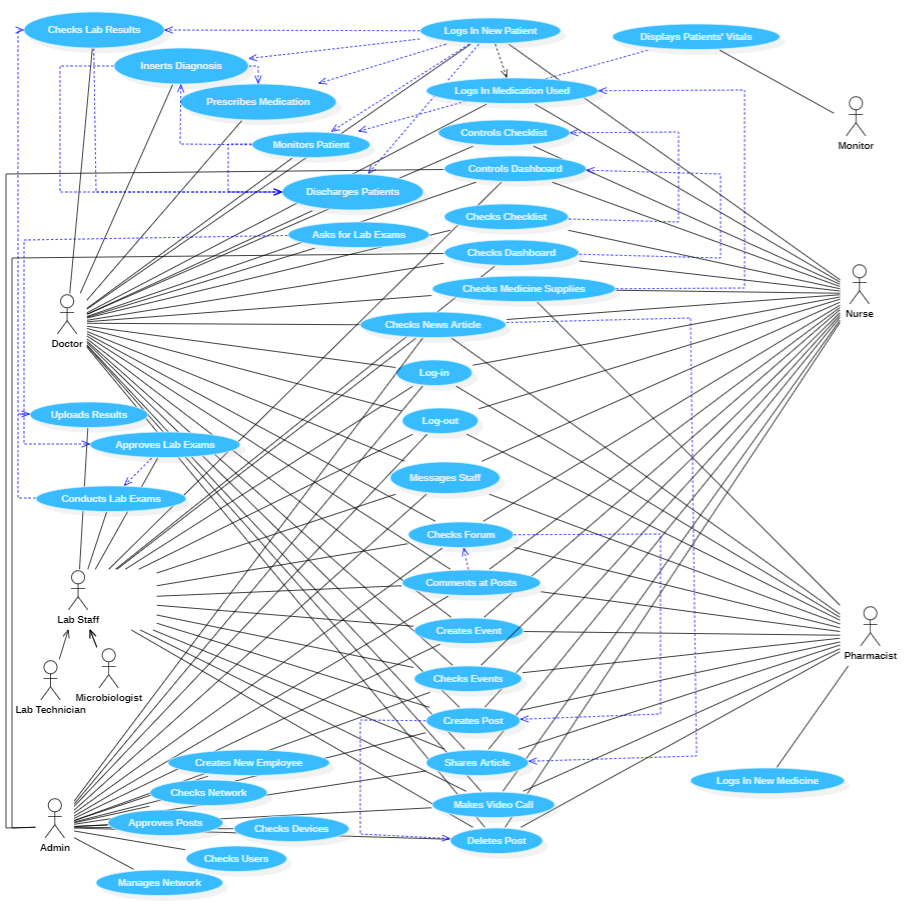
\includegraphics[width=1.1\textwidth]{UML.png}
        \caption{\label{fig: UML} Use Case Diagram}
\end{figure}

\vspace{0.2cm}

Από τις περιπτώσεις χρήσης του \textbf{Medic World}, που φαίνονται στο διάγραμμα, για τις δέκα, θα παρουσιαστούν παρακάτω αναλυτικές περιγραφές.

\newpage

\section{Use Case 1: Ενέργειες στην Καρτέλα Ασθενούς}

Παρακάτω θα αναλυθεί το σενάριο χρήσης του \textbf{Medic World}, στο οποίο ένας γιατρός πραγματοποιεί συγκεκριμένες αλλαγές στην καρτέλα ενός ασθενούς.

\subsection{Γενική Περιγραφή}

Εξαιτίας του γεγονότος ότι οι λειτουργίες που μπορούν να πραγματοποιηθούν μέσω της καρτέλα του ασθενούς είναι πολυάριθμες, αποφασίσαμε να αναλύσουμε δύο απο τις πιο σημαντικές, την εισαγωγή διάγνωσης και την έκδοση εξιτηρίου.
\par Καθώς τα βήματα των συγκεκριμένων περιπτώσεων χρήσης ως ένα σημείο ταυτίζονται, παρακάτω θα παρουσιαστεί ένας κοινός πίνακας με τα βήματα που είναι ίδια και για τα δύο και στη συνέχεια θα χωριστούν σε δύο διαφορετικά use cases. 

 \subsection{Γενικό Σενάριο Χρήσης}
 
 \begin{center}
     \begin{tabular}{|l|l|}
     \hline
      \textbf{Βήμα 1} & Ο γιατρός από το κεντρικό μενού επιλέγει να μεταφερθεί στις \T \\& καρτέλες των ασθενών \B \\
      \hline
      \textbf{Βήμα 2} &  Στο νέο παράθυρο το σύστημα εμφανίζει όλους τους ενεργούς ασθενείς \T \\& που νοσηλεύονται στο νοσοκομείο \B \\
      \hline
      \textbf{Βήμα 3} & Στο ίδιο παράθυρο επιλέγει τον ασθενή που χρειάζεται διάγνωση \T\B \\
      \hline
      \textbf{Βήμα 4} & Σε νέο παράθυρο εμφανίζονται οι τρέχουσες ζωτικές ενδείξεις του ασθενούς, \T \\& τα συμπτώματα του, αποτελέσματα από την ψιλάφιση/εξέταση, η ομάδα γιατρών \\& που τον παρακολουθεί, οι αλλεργίες του κ.ο.κ. \B \\
      \hline
      \textbf{Βήμα 5} & Ο γιατρός επιλέγει να ελέγξει το ιστορικό του ασθενούς \T\B \\
      \hline
      \textbf{Βήμα 6} & Σε νέα καρτέλα το σύστημα εμφανίζει τα δημογραφικά και κλινικά δεδομένα του \T\B \\
      \hline
      \textbf{Βήμα 7} & Μεταφορά στο σενάριο χρήσης "Εισαγωγή Διάγνωσης" ή "Έκδοση Εξιτηρίου\T\B \\
      \hline      
     
     \end{tabular}
 \end{center}
 
 \textbf{\underline{Εναλλακτική Ροή 1}: Επιτυχής Αναζήτηση Ασθενούς} \vspace{0.2cm}
\par \textbf{Βήμα 3.1:} Στην μπάρα αναζήτησης πληκτρολογεί το όνομα του ασθενούς και το σύστημα \par εμφανίζει προτάσεις με ασθενείς που είναι ήδη καταχωρημένοι και έχουν παρόμοιο όνομα με αυτό που \par πληκτρολογεί ο γιατρός.\vspace{0.1cm} 
\par Τα υπόλοιπα βήματα ταυτίζονται με τα βήματα 4 έως 7 της κανονικής ροής.

\vspace{0.2cm}

\textbf{\underline{Εναλλακτική Ροή 2}: Ανεπιτυχής Αναζήτηση Ασθενούς}
\vspace{0.2cm}
\par \textbf{Βήμα 3.2:}  Πληκτρολογεί το όνομα του ασθενούς και στην μπάρα αναζήτησης το σύστημα δεν \par εμφανίζει προτάσεις με ασθενείς που έχουν παρόμοιο όνομα με αυτό που πληκτρολογεί ο γιατρός. \vspace{0.1cm}
\par \textbf{Βήμα 4.2:} Το σύστημα εμφανίζει μήνυμα ότι δεν υπάρχει ασθενής με όνομα παρόμοιο με αυτό \par που αναζητεί ο γιατρός. \vspace{0.1cm}
\par \textbf{Βήμα 5.2:} Το σύστημα κλείνει την μπάρα αναζήτησης και εμφανίζει την οθόνη με τις καρτέλες \par των ασθενών. \vspace{0.1cm}

\par Τα υπόλοιπα βήματα ταυτίζονται με τα βήματα 4 έως 7 της κανονικής ροής. 

\newpage

\subsubsection{Εισαγωγή Διάγνωσης}
 
 \begin{center}
     \begin{tabular}{|l|l|}
     \hline
      \textbf{Περίπτωση Χρήσης 1.1} & Ο γιατρός εισάγει τη διάγνωση ενός ασθενούς \T\B \\ 
      \hline
      \textbf{Ηθοποιός} & Γιατρός \T\B \\
      \hline
      \textbf{Σενάριο Περίπτωσης Χρήσης} & Ένας από τους ασθενείς χρείαζεται διάγνωση, οπότε \T\\& ο γιατρός εισέρχεται στην καρτέλα του, μελετάει τα\\& αποτελέσματα των εξετάσεών και τα συμπτώματά του και \\& καταλήγει σε διάγνωση \B \\
      \hline
      \textbf{Αφορμή} & Ασθενής χρειάζεται διάγνωση \T\B \\
      \hline
      \textbf{Προαπαιτούμενο 1} & Να έχει καταχωρηθεί ο ασθενής στο σύστημα \T\B \\
      \hline
      \textbf{Προαπαιτούμενο 2} & Να είναι έτοιμα τα αποτελέσματα των εργαστηριακών εξετάσεων \T\B \\
      \hline
     \end{tabular}
 \end{center}
 
\vspace{0.2cm}
 
 \begin{center}
     \begin{tabular}{|l|l|}
     \hline
      \textbf{Περιγραφή} & Αυτό το σενάριο περιγράφει μια κατάσταση όπου χρειάζεται \T \\& η πλοήγηση σε τέσσερις καρτέλες, οι οποίες τελικά\\& οδηγούν στην επίτευξη του στόχου. \B \\ 
      \hline
      \textbf{Βήμα 8} & O γιατρός επιλέγει να εισάγει διάγνωση και εμφανίζεται σε αναδυόμενο \T \\& παράθυρο μια λίστα με πιθανές προτάσεις ασθενειών που ταιριάζουν στο \\& προφίλ του ασθενούς σύμφωνα με τα συμπτώματα και τις εξετάσεις του \B \\
      \hline
      \textbf{Βήμα 9} & Ο γιατρός επιλέγει την ασθένεια που ταυτίζεται με τη διάγνωσή του  \T\B \\
      \hline
      \textbf{Βήμα 10} & Σε νέα καρτέλα εμφανίζεται η προεπισκόπηση της διάγνωσης \T\B \\
      \hline
      \textbf{Βήμα 11} & Ο γιατρός καταχωρεί την διάγνωση του \T\B \\
      \hline
      \textbf{Βήμα 12} & Σε αναδυόμενο παράθυρο εμφανίζεται μήνυμα επιτυχίας \T\B \\
      \hline    
      \textbf{Βήμα 13} & Ενημερώνεται το σύστημα και το προφίλ του ασθενούς \T\B \\
      \hline
      \textbf{Βήμα 14} & Το σύστημα στέλνει ειδοποίηση στους υπόλοιπους γιατρούς \T \\& που έχουν καταχωρηθεί ως "care team" για τον συγκεκριμένο \\& ασθενή πως έχει γίνει ενημέρωση της διάγνωσής τελευταίου \B \\
      \hline
    \end{tabular}
 \end{center}
 
\textbf{\underline{Εναλλακτική Ροή 1:} Απόρριψη Προτάσεων}  \vspace{0.2cm}
\par \textbf{Βήμα 9.1.:} Δεν τον ικανοποιεί καθόλου η λίστα των πιθανών ασθενειών, επομένως \par "κλείνει" αυτό το παράθυρο. \vspace{0.1cm}
\par \textbf{Βήμα 10.1:} Κατευθύνεται απευθείας στο παράθυρο προεπισκόπησης της διάγνωσης. \vspace{0.1cm}
\par \textbf{Βήμα 11.1:} Εισάγει τη διάγνωση του. \vspace{0.1cm}

\par Τα υπόλοιπα βήματα ταυτίζονται με τα βήματα 11 έως 14 της κανονικής ροής.

\subsubsection{Έκδοση Εξιτηρίου}
 
 \begin{center}
     \begin{tabular}{|l|l|}
     \hline
      \textbf{Περίπτωση Χρήσης 1.2} & Ο γιατρός δίνει εξιτήριο σε κάποιον ασθενή \T\B \\ 
      \hline
      \textbf{Ηθοποιός} & Γιατρός \T\B \\
      \hline
      \textbf{Σενάριο Περίπτωσης Χρήσης} & Ένας από τους ασθενής ολοκλήρωσε τη θεραπεία του, οπότε \T\\& ο γιατρός εισέρχεται στην καρτέλα του για να του δώσει εξιτήριο \B \\
      \hline
      \textbf{Αφορμή} & Ασθενής χρειάζεται εξιτήριο \T\B \\
      \hline
      \textbf{Προαπαιτούμενο 1} & Να έχει καταχωρηθεί ο ασθενής στο σύστημα \T\B \\
      \hline
     \end{tabular}
 \end{center}
 
\newpage

 \begin{center}
     \begin{tabular}{|l|l|}
     \hline
      \textbf{Περιγραφή} & Αυτό το σενάριο περιγράφει μια κατάσταση όπου χρειάζεται \T \\& πλοήγηση σε τρεις καρτέλες, οι οποίες οδηγούν στην επίτευξη \\& του στόχου \B \\ 
      \hline
      \textbf{Βήμα 8} & Επιλέγει να εκδόσει εξιτήριο και σε νέο παράθυρο συμπληρώνει τα απαραίτητα \T \\& στοιχεία της φόρμας εξιτηρίου (medication και nutrition recommendations) \B \\
      \hline
      \textbf{Βήμα 9} & Επιλέγει να εκτυπώσει τη συγκεκριμένη φόρμα \T\B \\
      \hline
      \textbf{Βήμα 10} & Σε αναδυόμενο παράθυρο εμφανίζεται η τελική μορφή του εξιτηρίου και \T \\& οι διάφορες λειτουργίες/επιλογές εκτύπωσης (π.χ. εύρεση κοντινών εκτυπωτών) \B \\
      \hline
      \textbf{Βήμα 11} & Επιλέγει κάποιον από τους κοντινούς εκτυπωτές, δίνει έγκριση για \T \\& εκτύπωση και όταν αυτή ολοκληρωθεί, εμφανίζεται μήνυμα επιτυχίας \B \\
      \hline
      \textbf{Βήμα 12} & Επιστρέφει στο παράθυρο "Post-discharge Guidance" από το οποίο επιλέγει να \T \\& κοινοποιήσει μέσω ηλεκτρονικού ταχυδρομείου τις οδηγίες εξιτηρίου \B \\
      \hline
      \textbf{Βήμα 14} & Στο νέο παράθυρο εμφανίζεται η τελική μορφή του εξιτηρίου από το οποίο \T\\&επιβεβαίωνει την κοινοποίηση του \B \\
      \hline
      \textbf{Βήμα 15} & Στέλνεται αυτομάτως μήνυμα στο email που έχει καταχωρηθεί \T \\& για τον συγκεκριμένο ασθενή και εμφανίζεται μήνυμα επιτυχίας \B \\
      \hline
      \textbf{Βήμα 16} & Επιστρέφει στο παράθυρο "Post-discharge Guidance" και επιβεβαίωνει την \T \\&  έκδοση του εξιτηρίου  \B \\   
      \hline
      \textbf{Βήμα 17} & Εμφανίζεται μήνυμα επιτυχίας και ενημερώνονται κατάλληλα οι καρτέλες ασθενών  \T \B \\      
      \hline
      \textbf{Βήμα 18} & Το σύστημα στέλνει ειδοποίηση στους υπόλοιπους γιατρούς που έχουν \T \\& καταχωρηθεί ως "care team" για τον συγκεκριμένο ασθενή πως \\& εκδόθηκε εξιτήριο \B \\
      \hline
     \end{tabular}
 \end{center}
 
  \textbf{\underline{Εναλλακτική Ροή 1:} Συμπλήρωση Ηλεκτρονικού Ταχυδρομείου} \vspace{0.2cm}
\par \textbf{Βήμα 15.1:} Δεν έχει καταχωρηθεί e-mail για τον συγκεκριμένο ασθενή, συνεπώς οδηγείται σε \par αναδυόμενο παράθυρο, το οποίο ζητά από τον γιατρό την συμπλήρωση κάποιας διεύθυνσης \par ηλεκτρονικού ταχυδρομείου.

\vspace{0.2cm}

\par \textbf{Βήμα 16.1.α:} Ο Γιατρός εισάγει ένα email που πληροί τις προυϋποθέσεις και επιβεβαιώνει την \par καταχώρηση. \vspace{0.2cm}
\par \textbf{Βήμα 16.1.β:} Το email είναι λανθασμένο (δεν έχει τη μορφή ...@...com) και το σύστημα κλειδώνει \par την λειτουργία επιβεβαίωσης καταχώρησης εώς ότου εισαχθεί σωστό email. \vspace{0.1cm}

\par Τα υπόλοιπα βήματα ταυτίζονται με τα βήματα 15 έως 18 της κανονικής ροής.

\vspace{0.2cm}

 \textbf{\underline{Εναλλακτική Ροή 2:} Αδυναμία Διαδικασίας Εκτύπωσης} \vspace{0.2cm}
\par \textbf{Βήμα 11.2:} Για κάποιο λόγο δεν εμφανίζεται η λίστα των εκτυπωτών και παρουσιάζεται μήνυμα με \par την αιτία αδυναμίας της εκτύπωσης (βλάβη δικτύου, αδυναμία επικοινωνίας με τις \parσυσκευές, βλάβη στις συσκευές κ.ο.κ.).\vspace{0.1cm}
\par \textbf{Βήμα 12.2:} Πραγματοποιείται ακύρωση της διαδικασίας και το σύστημα τον επιστρέφει στην προ- \parηγούμενη καρτέλα (post-discharge guidance).

\newpage

\section{Use Case 2: Καταχώρηση Νέου Φαρμάκου }
 
 Παρακάτω θα αναλυθεί το σενάριο χρήσης του \textbf{Medic World} κατά το οποίο ένας φαρμακοποιός επιθυμεί να εισάγει στο σύστημα ένα νέο φάρμακο.
 
\subsection{Περιγραφή}

\begin{center}
     \begin{tabular}{|l|l|}
     \hline
      \textbf{Περίπτωση Χρήσης 3} & Ο χρήστης εισάγει νέο φάρμακο στην καρτέλα προμηθειών \T\B \\ 
      \hline
      \textbf{Ηθοποιός} & Φαρμακοποιός \T\B \\
      \hline
      \textbf{Σενάριο Περίπτωσης Χρήσης} & Έχει γίνει από το νοσοκομείο αγορά ενός νέου φαρμάκου \T \\& και ο φαρμακοποιός καλείται να το καταχωρήσει \\& στην καρτέλα προμηθειών \B \\
      \hline
      \textbf{Αφορμή} & Η αγορά νέου φαρμάκου \T\B \\
      \hline
      \textbf{Προαπαιτούμενο 1} &  Να μην υπάρχει ήδη το φάρμακο στην καρτέλα προμηθειών \T\B \\
      \hline
     \end{tabular}
 \end{center}
 
   \subsection{Αναλυτικό Σενάριο Χρήσης}
 
 \begin{center}
     \begin{tabular}{|l|l|}
     \hline
      \textbf{Περιγραφή} & Αυτό το σενάριο περιγράφει μια κατάσταση όπου χρειάζεται \T \\& πλοήγηση σε δύο καρτέλες, οι οποίες οδηγούν στην επίτευξη \\& του στόχου \B \\ 
      \hline
      \textbf{Βήμα 1} & Ο φαρμακοποιός από το κεντρικό μενού επιλέγει να μεταφερθεί στην \T \\& καρτέλα των προμηθειών \B \\
      \hline
      \textbf{Βήμα 2} & Στο νέο παράθυρο το σύστημα εμφανίζει όλες τις διαθέσιμες κατηγορίες \T \\& φαρμάκων του νοσοκομείου εκείνη την στιγμή \B \\
      \hline
      \textbf{Βήμα 3} & Στο ίδιο παράθυρο ο χρήστης επιλέγει την λειτουργεία "New Medicine" \T \\& (προσθήκη νέου φαρμάκου) \B \\
      \hline
      \textbf{Βήμα 4} & Σε νεό παράθυρο εμφανίζονται όλα τα πεδία που πρέπει να συμπληρώσει \T \\&  ο φαρμακοποιός για την καταχώριση νέου φαρμάκου. Πληκτρολογώντας τη \\& κατηγορία του φαρμάκου στον χρήστη εμφανίζονται προτάσεις από τις \\& υπάρχουσες κατηγορίες  (λ.χ. αντιβιοτικό), από τις οποίες επιλέγει κάποια \B \\
      \hline
      \textbf{Βήμα 5} & Στο ίδιο παράθυρο ο φαρμακοποιός καταχωρεί το όνομα του φαρμάκου \T\B \\
      \hline
      \textbf{Βήμα 6} &  Συμπληρώνει τα τεμάχια που έχει προμηθευτεί το νοσοκομείο \T\B \\
      \hline
      \textbf{Βήμα 7} & Καταγράφει τα όρια των τιμών που περιγράφουν την πληρότητα του \T \\& φαρμάκου (αν είναι σε αφθονία κ.ο.κ.)\B \\
      \hline
      \textbf{Βήμα 8} & Συμπληρώνει τα υποχρεωτικά πεδία και ολοκληρώνει τη διαδικασία \T \\& καταχώρησης φαρμάκου \B \\
      \hline
      \textbf{Βήμα 9} & Εμφανίζεται αναδυόμενο παράθυρο που υποδηλώνει την επιτυχία της διαδικασίας \T\B \\
      \hline    
      \textbf{Βήμα 10} & Γίνεται καταχώρηση στο σύστημα και ενημερώνεται κατάλληλα η καρτέλα \T \\& διαθεσιμότητας φαρμάκων \B \\
      \hline
     \end{tabular}
 \end{center}
 
  \textbf{\underline{Εναλλακτική Ροή 1:} Μη Καταχωρημένη Κατηγορία Φαρμάκου}  \vspace{0.1cm}
\par Η κατηγορία φαρμάκου που πληκτρολόγησε ο φαρμακοποιός δεν  αναγνωρίζεται από το σύστημα. \vspace{0.1cm}
\par \textbf{Βήμα 4.1:} Ο φαρμακοποιός ενημερώνεται πως η κατηγορία φαρμάκου που έχει πληκτρολογήσει, \parδεν υπάρχει στο σύστημα. \vspace{0.1cm}
\par Στη συνέχεια εισερχόμαστε στα βήματα 5, 6, 7, 8 και 9 της κανονικής ροής. \vspace{0.1cm}
\par \textbf{Βήμα 10.1:} Δημιουργείται αυτόματα νέα κατηγορία στο σύστημα, γίνεται καταχώρηση και \par ενημερώνεται κατάλληλα η καρτέλα διαθεσιμότητας φαρμάκων.

\vspace{0.2cm}
 
\textbf{\underline{Εναλλακτική Ροή 2:} Προσθήκη Ήδη Καταχωρημένου Φαρμάκου} \vspace{0.2cm} 
\par \textbf{Βήμα 5.2:} Το φάρμακο που συμπλήρωσε ο φαρμακοποιός είναι ήδη καταχωρημένο, με αποτέλεσμα \par να μην του επιτρέπεται η συνέχεια της διαδικασίας εώς ότου διορθωθεί το όνομα.\vspace{0.1cm}

\vspace{0.2cm}

\textbf{\underline{Εναλλακτική Ροή 3:} Μη Συμπλήρωση Υποχρεωτικών Πεδίων} \vspace{0.2cm} 
\par \textbf{Βήμα 8.4:} Ο φαρμακοποιός δεν έχει συμπληρώσει τα πεδία που είναι υποχρεωτικά για την καταχώρηση \par του φαρμάκου. Το σύστημα δεν επιτρέπει τη συνέχεια της διαδικασίας και αποκρίνεται με μήνυμα \par που επεξηγεί το λόγο. \vspace{0.2cm}

\textbf{\underline{Εναλλακτική Ροή 4:} Εσφαλμένη Συμπλήρωση Πεδίων} \vspace{0.2cm} 
\par \textbf{Βήμα 6.5/Βήμα 7.5:} Η συμπλήρωση των πεδίων δεν είναι σωστή (τα πεδία δεν περιέχουν μόνο \par ψηφία). Το σύστημα δεν επιτρέπει την συνέχεια της διαδικασίας και αποκρίνεται με μήνυμα που \par επεξηγεί το λόγο.

 \section{Use Case 3: Απασχόληση Χειρουργείου}
 
 Παρακάτω θα αναλυθεί το σενάριο χρήσης του \textbf{Medic World}, στο οποίο ένας χρήστης επιθυμεί να δηλώσει στο σύστημα τη χρήση ενός χειρουργείου.

\subsection{Περιγραφή}

\begin{center}
     \begin{tabular}{|l|l|}
     \hline
      \textbf{Περίπτωση Χρήσης 2} & Ο χρήστης δηλώνει την απασχόληση χειρουργείου \T\B \\ 
      \hline
      \textbf{Ηθοποιός} & Γιατρός \T\B \\
      \hline
      \textbf{Σενάριο Περίπτωσης Χρήσης} & Ένας γιατρός πρόκειται να εισάγει έναν ασθενή \T \\& σε κάποιο χειρουργείο και χρειάζεται να καταχωρηθεί\\& στην καρτέλα των χειρουργείων ότι το συγκεκριμένο\\& δωμάτιο δε θα είναι διαθέσιμο για κάποιο χρονικό διάστημα \B \\
      \hline
      \textbf{Ηθοποιοί} & Γιατρός, Νοσηλευτής \T\B \\
      \hline
      \textbf{Αφορμή} & Ασθενής χρειάζεται χειρουργείο \T\B \\
      \hline
      \textbf{Προαπαιτούμενο 1} & Να έχει καταχωρηθεί ο ασθενής στο σύστημα \T\B \\
      \hline
      \textbf{Πρoαπαιτούμενο 2} & Να έχει πραγματοποιηθεί διάγνωση του ασθενούς \T\B \\
      \hline
      \textbf{Προαπαιτούμενο 3} & Η διάγνωση να απαιτεί την εισαγωγή σε χειρουργείο \T\B \\
      \hline
     \end{tabular}
 \end{center}
 
   \subsection{Αναλυτικό Σενάριο Χρήσης}
 
 \begin{center}
     \begin{tabular}{|l|l|}
     \hline
      \textbf{Περιγραφή} & Αυτό το σενάριο περιγράφει μια κατάσταση όπου χρείαζεται η πλοήγηση σε τρεις καρτέλες, \T \\& οι οποίες οδηγούν στην επίτευξη του στόχου. \B \\ 
      \hline
      \textbf{Βήμα 1} & Ο γιατρός από το κεντρικό μενού επιλέγει να μεταφερθεί στην καρτέλα διαθεσιμότητας \T \\& δωματίων \B \\
      \hline
      \textbf{Βήμα 2} & Επιλέγει να ελέγξει την διαθεσιμότητα των χειρουργείων \T\B \\ 
      \hline
      \textbf{Βήμα 3} & Σε νέο παράθυρο εμφανίζονται όλα τα χειρουργεία, διαθέσιμα και μη, με τις αντίστοιχες ενδείξεις \T \\& (γιατρός που χειρουργεί, εγχείρηση που λαμβάνει χώρα κ.ο.κ.) \B \\
      \hline
      \textbf{Βήμα 4} & Ο γιατρός επιλέγει κάποιο από τα διαθέσιμα χειρουργεία \T\B \\
      \hline
      \textbf{Βήμα 5} & Σε νέα καρτέλα εμφανίζεται η φόρμα συμπλήρωσης των απαραίτητων στοιχείων \T\B \\
      \hline
      \textbf{Βήμα 6} & Για τη συμπλήρωση των στοιχείων όνομα ασθενούς, γιατρού και εγχείρησης \T \\& πληκτρολογώντας στο αντίστοιχο πεδίο κάθε φορά εμφανίζονται προτάσεις, \\& σύμφωνα με το κείμενο που πληκτρολογεί ο γιατρός \B \\
      \hline      
      \textbf{Βήμα 7} & Συμπληρώνει τα υποχρεωτικά πεδία και ολοκληρώνει την διαδικασία\T\B \\
      \hline
      \textbf{Βήμα 8} & Εμφανίζεται αναδυόμενο παράθυρο με την ένδειξη "Successful" \T\B \\
      \hline
      \textbf{Βήμα 9} & Ενημερώνεται κατάλληλα το σύστημα και η καρτέλα διαθεσιμότητας των χειρουργείων \T\B \\
      \hline
     \end{tabular}
 \end{center}
 
  \textbf{\underline{Εναλλακτική Ροή 1:} Ανεπιτυχής Αναζήτηση Γιατρού} \vspace{0.2cm} 
\par \textbf{Βήμα 6.1:} Πληκτρολογεί το όνομα του γιατρού και στην μπάρα αναζήτησης το σύστημα δεν \par εμφανίζει προτάσεις με γιατρούς που έχουν παρόμοιο όνομα με αυτό που πληκτρολόγησε. \vspace{0.1cm}
\par \textbf{Βήμα 7.1:} Εμφανίζεται κατάλληλο μήνυμα αποτυχίας και δεν επιτρέπεται στον γιατρό να προχωρήσει \par με την διαδικασία, μέχρι να επιλέχθει κάποιο από το ονόματα που προτείνεται από τη λίστα.\vspace{0.1cm}
\par Συμπληρώνει τα κατάλληλα στοιχεία και τα βήματα της εναλλακτικής ροής 1, πλέον, ταυτίζονται με \par τα βήματα 7 εως 9 της κανονικής ροής. \vspace{0.2cm}

\textbf{\underline{Εναλλακτική Ροή 2:} Εσφαλμένη Επιλογή Γιατρού} \vspace{0.2cm} 

\par \textbf{Βήμα 6.2:} Ο συγκεκριμένος γιατρός βρίσκεται σε άλλο απασχολημένο χειρουργείο. Το σύστημα \par δεν επιτρέπει την ολοκλήρωση της διαδικασίας και εμφανίζει μήνυμα που επεξηγεί το λόγο. \vspace{0.2cm}

\textbf{\underline{Εναλλακτική Ροή 3:} Μη Συμπλήρωση Υποχρεωτικών Πεδίων} \vspace{0.2cm} 
\par \textbf{Βήμα 7.3:} Ο γιατρός δεν έχει συμπληρώσει τα πεδία που είναι υποχρεωτικά για την απασχόληση \par του χειρουργείου. Το σύστημα δεν επιτρέπει τη συνέχεια της διαδικασίας και αποκρίνεται με μήνυμα \par που επεξηγεί το λόγο.\vspace{0.2cm}

\section{Use Case 4: Αποστολή Μηνύματος}

Παρακάτω θα αναλυθεί το σενάριο χρήσης του \textbf{Medic World}, στο οποίο ένας χρήστης της εφαρμογής επιθυμεί να στείλει μήνυμα σε κάποιον άλλο χρήστη.

\subsection{Περιγραφή}

\begin{center}
     \begin{tabular}{|l|l|}
     \hline
      \textbf{Περίπτωση Χρήσης 4} & Ο χρήστης στέλνει μήνυμα σε κάποιον άλλο χρήστη της εφαμοργής \T\B \\ 
      \hline
      \textbf{Ηθοποιός} & Γιατρός \T\B \\
      \hline
      \textbf{Σενάριο Περίπτωσης Χρήσης} & Έχει εισαχθεί ένας νέος ασθενής στο νοσοκομείο και επιθυμεί να \T \\& μάθει, αν ένας συνάδελφός του έχει ελέγξει τις εξετάσεις \B \\
      \hline
      \textbf{Ηθοποιοί} & Γιατρός, Νοσηλευτής, Μικροβιολόγος, Υπεύθυνοι Εργαστηρίου, \T \\& Φαρμακοποιός, Διαχειριστής Συστήματος \T\B \\
      \hline
      \textbf{Αφορμή} & Έτοιμες εξετάσεις για έλεγχο \T\B \\
      \hline
      \textbf{Προαπαιτούμενο 1} & Να έχει εισαχθεί ο ασθενής στο σύστημα \T\B \\
      \hline
      \textbf{Προαπαιτούμενο 2} & Να έχει γίνει η παραγγελία των εξετάσεων \T\B \\
      \hline
      \textbf{Προαπαιτούμενο 3} & Να έχουν ολοκληρωθεί οι εξετάσεις \T\B \\
      \hline
     \end{tabular}
 \end{center}
 
  \newpage
 
 \subsection{Αναλυτικό Σενάριο Χρήσης}

 \begin{center}
     \begin{tabular}{|l|l|}
     \hline
      \textbf{Περιγραφή} & Αυτό το σενάριο περιγράφει μια κατάσταση όπου χρειάζεται \T \\& πλοήγηση σε τρεις καρτέλες, οι οποίες οδηγούν στην επίτευξη \\& του στόχου \B \\ 
      \hline
      \textbf{Βήμα 1} & Ο γιατρός από το κεντρικό μενού επιλέγει να μεταφερθεί στην \T \\& καρτέλα των μηνυμάτων \B \\
      \hline
      \textbf{Βήμα 2} & Στο νέο παράθυρο το σύστημα εμφανίζει το ιστορικό όλων των \T \\& συζητήσεων του γιατρού με τους υπόλοιπους χρήστες της εφαρμογής \B \\
      \hline
      \textbf{Βήμα 3} & Ανανεώνεται το status του γιατρού και πλέον φαίνεται ενεργός \T\B \\
      \hline
      \textbf{Βήμα 4} & Ο γιατρός επιλέγει τη σύνταξη καινούργιου μήνυματος \T\B \\
      \hline
      \textbf{Βήμα 5} & Σε νέο παράθυρο πληκτρολογώντας το όνομα του χρήστη, εμφανίζονται προτάσεις \T \\& από τους ήδη εγγεγραμμένους χρήστες, από τους οποίους επιλέγει κάποιον  \B \\
      \hline
      \textbf{Βήμα 6} & Κατευθύνεται σε νέο παράθυρο στο οποίο το σύστημα φορτώνει τη συζήτηση με τον \T \\& συγκεκριμένο χρήστη και τις διάφορες λειτουργίες αποστολής μηνύματος, όπως \\& είναι η αποστολή φωτογραφίας, δημιουργία βιντεοκλήσης κ.ο.κ  \B \\
      \hline
      \textbf{Βήμα 7} & Πληκτρολογεί και αποστέλλει ένα μήνυμα \T\B \\
      \hline
      \textbf{Βήμα 8} & Το σύστημα ανανεώνει τη συζήτηση μεταξύ των δύο χρηστών λόγω της \T \\& αποστολής καινούργιου μηνύματος \B \\
      \hline
      \textbf{Βήμα 9} & Το σύστημα ενημερώνει τον χρήστη για την κατάσταση αποστολής του μηνύματος \T \\& (εάν έχει σταλεί επιτυχώς, εάν έχει ληφθεί από τον παραλήπτη κ.ο.κ.) \B \\
      \hline
      \textbf{Βήμα 10} & Η κατάσταση του μηνύματος ενημερώνεται, αφού ο παραλήπτης το διαβάσει \T\B \\
      \hline
     \end{tabular}
 \end{center}
 
\textbf{\underline{Εναλλακτική Ροή 1:} Επιλογή Πρόσφατης Συνομιλίας} \vspace{0.2cm}
\par\textbf{Βήμα 5.1:} Ο χρήστης που επιθυμεί να συνομιλήσει, βρίσκεται ήδη στο ιστορικό των συζητήσεων \par του, επομένως περιηγείται στην οθόνη και παρατηρεί πως έχουν ήδη συνομιλήσει, συνεπώς επιλέγει \par την συνομιλία τους.  \vspace{0.1cm}

\par Τα υπόλοιπα βήματα ταυτίζονται με τα βήματα 6 έως 9 της κανονικής ροής. \vspace{0.2cm}

\textbf{\underline{Εναλλακτική Ροή 2:} Ανεπιτυχής Αναζήτηση Χρήστη} \vspace{0.2cm}
\par \textbf{Βήμα 5.2:} Πληκτρολογεί το όνομα του χρήστη και στην μπάρα αναζήτησης το σύστημα δεν \par εμφανίζει προτάσεις με χρήστες που έχουν παρόμοιο όνομα με αυτό που πληκτρολογεί ο γιατρός. \vspace{0.1cm}
\par \textbf{Βήμα 6.2:} Εμφανίζεται μήνυμα αποτυχίας εύρεσης κάποιου χρήστη της εφαρμογής. \vspace{0.1cm}

\section{Use Case 5: Έγκριση και Διεξαγωγή Εξετάσεων}

Παρακάτω θα αναλυθεί το σενάριο χρήσης του \textbf{Medic World}, στο οποίο ο υπεύθυνος εργαστηρίου καλέιται να πραγματοποιήσει κάποποιες εξετάσεις.

\subsection{Περιγραφή}

\begin{center}
     \begin{tabular}{|l|l|}
     \hline
      \textbf{Περίπτωση Χρήσης 10} & Ο υπεύθυνος του μικροβιολογικού εργαστήριου καλείται να διεξάγει\T\\& μία σειρά εξετάσεων\B \\ 
      \hline
      \textbf{Ηθοποιός} & Υπεύθυνος Εργαστηρίου (Μικροβιολογικού) \T\B \\
      \hline
      \textbf{Σενάριο Περίπτωσης Χρήσης} & Για έναν ασθενή γίνεται αίτητση από έναν γιατρό για διεξαγωγή σειράς\T\\& εξετάσεων και ο υπεύθυνος του μικροβιολογικού καλείται να τις εκπονήσει\B\\
      \hline
      \textbf{Ηθοποιοί} & Γιατρός, Υπεύθυνος Εργαστηρίου \T\B \\
      \hline
      \textbf{Αφορμή} &  Αίτηση για διεξαγωγή εξετάσεων σε ασθενή\T\B \\
      \hline
     \end{tabular}
 \end{center}
 
  \subsection{Αναλυτικό Σενάριο Χρήσης}
 
  \begin{center}
     \begin{tabular}{|l|l|}
     \hline
      \textbf{Περιγραφή} & Αυτό το σενάριο περιγράφει μια κατάσταση όπου χρειάζεται \T \\& πλοήγηση σε τρεις καρτέλες, οι οποίες οδηγούν στην επίτευξη \\& του στόχου \B \\ 
      \hline
      \textbf{Βήμα 1} & Ο υπεύθυνος εργαστηρίου βρίσκεται στο κεντρικό μενού (Dashboard) και \T \\& εμφανίζεται ειδοποίηση ότι ένας γιατρός ζήτησε τη διεξαγωγή ορισμένων \\& μικροβιολογικών ελέγχων για έναν ασθενή\B \\
      \hline
      \textbf{Βήμα 2} & Από το ίδιο παράθυρο επιλέγει την ειδοποίηση και εμφανίζεται αναδυόμενο \T \\& παράθυρο για την έγκριση του αιτήματος\B\\
      \hline
      \textbf{Βήμα 3} & Εγκρίνει την αίτηση και το σύστημα τον μεταφέρει αυτόματα στην καρτέλα \T \\& διαχείρισης εργαστηριακών μονάδων της καρτέλας "Checklist"\B \\
      \hline
      \textbf{Βήμα 4} & Επιλέγει εργαστηριακή μονάδα και συμπληρώνει το πεδίο "Τεχνικός Εργαστηρίου"\T\\& ενώ πληκτρολογώντας το σύστημα εμφανίζει προτάσεις με τους ήδη καταχωρημένους \\& Τεχνικούς Εργαστηρίου ενώ το πεδίο του ασθενούς συμπληρώνεται αυτόματα  \B \\
      \hline
      \textbf{Βήμα 5} & Επιλέγει την ώρα που θα κατοχυρώσει το εργαστήριο και γίνεται έλεγχος \T\\& διαθεσιμότητας για την ώρα που επιθυμεί και το σύστημα εμφανίζει ένδειξη \\& επιτυχίας για τη συγκεκριμένη ώρα\B\\
      \hline
      \textbf{Βήμα 6} & Επιλέγει την ολοκλήρωση της διαδικασίας, πραγματοποιείται έλεγχος του συστήματος \T \\& για τα συμπληρωμένα υποχρεωτικά πεδία και εμφανίζεται μήνυμα επιτυχίας ολοκλήρωσης \\& της κατοχύρωσης \B\\
      \hline
      \textbf{Βήμα 7} & Ενημερώνεται κατάλληλα η καρτέλα διαθεσιμότητας των εργαστηρίων, εμφανίζοντας\T\\& πλέον ότι για την ώρα που ζητήθηκε το εργαστήριο θα έχει κατοχύρωθεί από το \\&  συγκεκριμένο υπεύθυνο εργαστηρίου\B \\
      \hline
      \textbf{Βήμα 8} &  Ανάλογα με το προφίλ του ασθενούς και την παραγγελία των εξετάσων, που \T\\& πραγματοποίησε ο γιατρός, σε καινούργιο παράθυρο το σύστημα προτείνει στον \\& μικροβιολόγο μία λίστα από τα πειράματα και τις διεργασίες που πρέπει να \\& ακολουθήσει για τη διεξαγωγή των συγκεκριμένων εργαστηριακών ελέγχων και ο \\& υπεύθυνος εργαστηρίου επιλέγει "ολοκλήρωση"\B \\
      \hline
      \textbf{Βήμα 9} & Κατά τη διάρκεια διεξαγωγής των εργαστηριακών ελέγχων, κάθε φορά που ο υπεύθυνος \T\\& ολοκληρώνει κάποιο από τα πειράματά του, το επιλέγει από τη λίστα του βήματος 8  και \\& το σύστημα στέλνει αυτόματα ειδοποίηση στον αιτούντα ιατρό για την εξέλιξη των \\& εξετάσεων μαζί με μία πρόβλεψη για το χρόνο που απομένει για την ολοκλήρωση τους \B \\
      \hline
      \textbf{Βήμα 10} & Ολοκληρώνεται ο εργαστηριακός έλεγχος, ο υπεύθυνος προσθέτει σχόλια για τα \T\\& αποτελέσματα και επιλέγει την αποστολή των αποτελεσμάτων\B \\
      \hline
      \textbf{Βήμα 11} & Το σύστημα ενημερώνει την καρτέλα του συγκεκριμένου ασθενούς με τα αποτελέσματα\T\\& των εξετάσεων και παράλληλα στέλνει ειδοποίηση στον αιτούντα ιατρό για την ολοκλήρωση \\& των εξετάσεων \B \\
      \hline
      \textbf{Βήμα 12} & Το σύστημα εμφανίζει μήνυμα επιβεβαίωσης για λήξη της κατοχύρωσης του εργαστηρίου \T\\& και ο υπεύθυνος επιλέγει "έγκριση"\B \\
      \hline
      \textbf{Βήμα 13} & Ενημερώνονται κατάλληλα οι καρτέλες διαθεσιμότητας των εργαστηριακών μονάδων,\T\\& εμφανίζοντας πλέον ότι το συγκεκριμένο εργαστήριο είναι διαθέσιμο για νέα κατοχύρωση\B \\
      \hline
     \end{tabular}
 \end{center}
 
  \textbf{\underline{Εναλλακτική Ροή 1:} Απόρριψη Διεξαγωγής Εξετάσεων} \vspace{0.2cm}
\par \textbf{Βήμα 3.1:} Απορρίπτει την αίτηση, το σύστημα αυτόματα ανακατευθύνει την αίτηση σε κάποιον άλλο \par υπεύθυνο εργαστηρίου του συγκεκριμένου κλάδου και στέλνει στον αιτούντα ιατρό μήνυμα \par ενημέρωσης. \vspace{0.2cm}

\textbf{\underline{Εναλλακτική Ροή 2:} Εσφαλμένη Συμπλήρωση Πεδίων} \vspace{0.2cm}
\par \textbf{Βήμα 4.2:} Ο υπεύθυνος συμπλήρωσε το πεδίο του Τεχνικού Εργαστηρίου με μη καταχωρημένο \par πρόσωπο, συνεπώς το σύστημα εμφανίζει κατάλληλο μήνυμα ενημέρωσης και δεν του επιτρέπει τη \par συνέχεια της διαδικασίας κατοχύρωσης \vspace{0.2cm}

\textbf{\underline{Εναλλακτική Ροή 3:} Μη Διαθέσιμο Εργαστήριο} \vspace{0.2cm}
\par \textbf{Βήμα 5.3:} Επιλέγει την ώρα που θα κατοχυρώσει το εργαστήριο, γίνεται έλεγχος διαθεσιμότητας \par και το σύστημα εμφανίζει κατάλληλο μήνυμα αποτυχίας της κατοχύρωσης εξηγώντας ότι το εργαστήριο \par δε βρίσκεται σε διαθεσιμότητα για την ώρα που επιθυμεί. \vspace{0.2cm}

\textbf{\underline{Εναλλακτική Ροή 4:} Μη Συμπλήρωση Υποχρεωτικών Πεδίων} \vspace{0.2cm}
\par \textbf{Βήμα 6.4:} Ο υπεύθυνος εργαστηρίου δεν έχει συμπληρώσει τα πεδία που είναι υπο- \par χρεωτικά για την καταχώριση του εργαστηρίου. Το σύστημα δεν επιτρέπει τη συνέχεια της διαδικασίας \par και αποκρίνεται με μήνυμα που επεξηγεί το λόγο.  \vspace{0.2cm}

\textbf{\underline{Εναλλακτική Ροή 5:} Τροποποίηση Λίστας Προτάσεων} \vspace{0.2cm}
\par \textbf{Βήμα 8.5:} Ο υπεύθυνος εργαστηρίου τροποποιεί την λίστα που εμφανίστηκε, προσθέτοντας μια \par διαφορετική πειραματική διαδικασία από τις ήδη προτεινόμενες. \vspace{0.1cm}
\par \textbf{Βήμα 9.5:} Στο ίδιο παράθυρο επιλέγει την ολοκλήρωση τροποποίησης της λίστας. \vspace{0.1cm}

\par Τα υπόλοιπα βήματα της εναλλακτικής ροής ταυτίζονται με τα βήματα 8 έως 12 της κανονικής ροής.

\section{Use Case 6: Έγκριση Δημοσίευσης}

Παρακάτω θα αναλυθεί το σενάριο χρήσης του \textbf{Medic World}, στο οποίο ο διαχειριστής επιθυμεί να εγκρίνει μια δημοσίευση προκειμένου να "ανέβει" στο "Community Forum".

\subsection{Περιγραφή}

\begin{center}
     \begin{tabular}{|l|l|}
     \hline
      \textbf{Περίπτωση Χρήσης 8} & Ο διαχεριστής συστήματος καλείται να δώσει έγκριση \T \\& σε μία δημοσίευση που έχει δημιουργηθεί στο "Community Forum". \B \\ 
      \hline
      \textbf{Ηθοποιός} & Διαχεριστής Συστήματος\T\B \\
      \hline
      \textbf{Σενάριο Περίπτωσης Χρήσης} & Ένας χρήστης της εφαρμογής επιθυμεί να δημοσιεύσει ένα post, \T \\&  το οποίο πρέπει να λάβει έγκριση από το διαχειριστή συστήματος\B \\
      \hline
      \textbf{Αφορμή} & Έχει δημιουργηθεί μία καινούργια δημοσίευση\T\B \\
      \hline
     \end{tabular}
 \end{center}
 
 \subsection{ Αναλυτικό Σενάριο Χρήσης}
 
  \begin{center}
     \begin{tabular}{|l|l|}
     \hline
      \textbf{Περιγραφή} & Αυτό το σενάριο περιγράφει μια κατάσταση όπου χρειάζεται \T \\& πλοήγηση σε τρεις καρτέλες, οι οποίες οδηγούν στην επίτευξη \\& του στόχου \B \\ 
      \hline
      \textbf{Βήμα 1} & Ο διαχεριστής συστήματος από το κεντρικό μενού επιλέγει να μεταφερθεί στην \T \\& καρτέλα "Newsroom" \B \\
      \hline
      \textbf{Βήμα 2} & Στο νέο παράθυρο εμφανίζεται η καρτέλα "News Article" ως προεπιλογή, \T \\& στην οποία το σύστημα παρουσιάζει τις πρόσφατες δημοσιεύσεις από \\& διάφορα εγκεκριμένες ιατρικές ιστοσελίδες \B \\
      \hline
      \textbf{Βήμα 3} & Επιλέγει την καρτέλα "Community Forum" \T\B \\
      \hline
      \textbf{Βήμα 4} & Σε νέα οθόνη εμφανίζονται όλα τα post που έχουν ήδη δημοσιευθεί, η δυνατότητα \T \\&  δημιουργίας νέας δημοσίευσης και όλα τα post που βρίσκονται σε λίστα αναμονής \\& προς έγκριση  \B \\
      \hline
      \textbf{Βήμα 5} & Επιλέγει τη λίστα με τα post που δεν έχουν ακόμη εγκριθεί και σε νέα καρτέλα  \T \\& εμφανίζονται όλες οι δημοσιεύσεις που απαιτούν έγκριση\B \\
      \hline
      \textbf{Βήμα 6} & Επιλέγει κάποια δημοσίευση και αυτή εμφανίζεται σε νέο παράθυρο  \T\B \\
      \hline
      \textbf{Βήμα 7} & Εισάγει μια βαθμολογία (υπό τη μορφή "άστρων" - 0 εώς 5) που αφορά \T \\& τον χρήστη, η οποία υποδεικνύει κατά πόσο η συγκεκριμένη δημοσίευση \\& είναι χρήσιμη και επιβεβαιώνει την έγκρισή της \B \\
      \hline
      \textbf{Βήμα 8} & Ενημερώνονται αφενός οι δημοσιευμένες αναρτήσεις και πλέον στην καρτέλα \T \\&  "Community Forum" εμφανίζεται η συγκεκριμένη δημοσίευση του χρήστη \\&  και αφετέρου η ουρά δημοσιεύσεων προς έγκριση\B \\
      \hline
     \end{tabular}
 \end{center}
 
  \textbf{\underline{Εναλλακτική Ροή 1:} Απόρριψη Δημοσίευσης } \vspace{0.2cm}
\par \textbf{Βήμα 7.1:} Δεν εγκρίνει την δημοσίευση. \vspace{0.1cm}
\par \textbf{Βήμα 8.1:} Αυτομάτως εμφανίζεται αναδυόμενο παράθυρο, στο οποίο μπορεί να προσθέσει το λόγο \par που δεν εγκρίθηκε το post. \vspace{0.2cm}

\par \textbf{Βήμα 9.1:} Επιλέγει επιβεβαίωση και η δημοσίευση δεν "ανεβαίνει" στο Community Forum. \vspace{0.1cm}
\par \textbf{Βήμα 10.1:}  Στέλνεται αυτομάτως μήνυμα στον χρήστη που υπέβαλλε τη δημοσίευση, το οποίο \par τον ενημερώνει για την απόρριψη της τελευταίας. \vspace{0.2cm}

\textbf{\underline{Εναλλακτική Ροή 2:} Εσφαλμένη Βαθμολόγηση} \vspace{0.2cm}
\par \textbf{Βήμα 7.2:} Η βαθμολογία είναι εκτός των ορίων. Το σύστημα δεν επιτρέπει την έγκριση της \par δημοσίευσης και αποκρίνεται με μήνυμα που επεξηγεί το λόγο. \vspace{0.2cm}

\textbf{\underline{Εναλλακτική Ροή 3:} Ενημέρωση Ηλεκτρονικών Παρασήμων} \vspace{0.2cm}
\par \textbf{Βήμα 7.3:} Ο χρήστης έχει λάβει πολλές καλές βαθμολογίες, όσον αφορά στις δημοσιεύσεις του που \par έχουν αναρτηθεί, συνεπώς το σύστημα ενημερώνει το status του ηλεκτρονικού του παρασήμου.

\section{Use Case 7: Δημιουργία Δημοσίευσης}

Παρακάτω θα αναλυθεί το σενάριο χρήσης του \textbf{Medic World}, στο οποίο ο γιατρός επιθυμεί να δημιουργήσει ένα post στο "Community Forum".

\subsection{Περιγραφή}

\begin{center}
     \begin{tabular}{|l|l|}
     \hline
      \textbf{Περίπτωση Χρήσης 8} & Ο γιατρός δημιουργεί ένα post στο Community Forum \T\B \\ 
      \hline
      \textbf{Ηθοποιός} & Γιατρός \T\B \\
      \hline
      \textbf{Σενάριο Περίπτωσης Χρήσης} & Ένας γιατρός στο νοσοκομείο επιθυμεί να κάνει μία ερώτηση \T \\& στο Forum σχετικά με μία συνάντηση που πρόκειται να \\& πραγματοποιηθεί στο νοσοκομειακό χώρο \B \\
      \hline
      \textbf{Ηθοποιοί} & Γιατρός, Νοσηλευτής, Μικροβιολόγος, Υπεύθυνοι Εργαστηρίου, \T \\& Φαρμακοποιός, Διαχειριστής Συστήματος \B \\
      \hline
      \textbf{Αφορμή} &  Ο γιατρός έχει μία απορία\T\B \\
      \hline
     \end{tabular}
 \end{center}
 
  \subsection{Αναλυτικό Σενάριο Χρήσης}

 \begin{center}
     \begin{tabular}{|l|l|}
     \hline
      \textbf{Περιγραφή} & Αυτό το σενάριο περιγράφει μια κατάσταση όπου χρειάζεται \T \\& πλοήγηση σε τρεις καρτέλες, οι οποίες οδηγούν στην επίτευξη \\& του στόχου \B \\ 
      \hline
      \textbf{Βήμα 1} & Ο γιατρός από το κεντρικό μενού επιλέγει να μεταφερθεί στην \T \\& καρτέλα "Newsroom" \T\B \\
      \hline
      \textbf{Βήμα 2} & Στο νέο παράθυρο εμφανίζεται η καρτέλα "News Article" ως προεπιλογή, \T \\& στην οποία το σύστημα παρουσιάζει τις πρόσφατες δημοσιεύσεις από \\& διάφορα εγκεκριμένες ιατρικές ιστοσελίδες \B \\
      \hline
      \textbf{Βήμα 3} & Στο ίδιο παράθυρο επιλέγει την καρτέλα "Community Forum" \T\B \\
      \hline
      \textbf{Βήμα 4} & Σε νέα οθόνη εμφανίζονται όλα τα post που έχουν ήδη δημοσιευθεί, καθώς \T \\& και η δυνατότητα δημιουργίας νέας δημοσίευσης \B \\
      \hline
      \textbf{Βήμα 5} & Επιλέγει να δημιουργήσει ένα καινούργιο post \T\B \\
      \hline
      \textbf{Βήμα 6} & Σε νέα καρτέλα εμφανίζονται όλες οι δυνατότητες επεξεργασίας δημοσίευσης,\T \\& όπως είναι η λήψη/προσθήκη φωτογραφίας, αναφορά σε κάποιο event κ.ο.κ. \B \\
      \hline
      \textbf{Βήμα 7} & Στο ίδιο παράθυρο γράφει κείμενο ($\le$ 280 χαρακτήρων) \T\B \\
      \hline
      \textbf{Βήμα 8} & Ανεβάζει μια φωτογραφία ($\le$60MB) \T\B \\
      \hline
      \textbf{Βήμα 9} & Ο Γιατρός ολοκληρώνει την δημοσίευση του και περιμένει να εγκριθεί \T \\& από τον διαχειριστή συστήματος \B \\
      \hline      
     \end{tabular}
 \end{center}
 
Στη συνέχεια πραγματοποιείται μετάβαση στην Περίπτωση Χρήσης "Έγκριση Δημοσίευσης".\vspace{0.2cm}

\textbf{\underline{Εναλλακτική Ροή 1:} Ενημέρωση για Απόρριψη Δημοσίευσης} \vspace{0.2cm}
\par \textbf{Βήμα 9.1:} Η δημοσίευση δεν εγκρίθηκε από το διαχειριστή του στυστήματος και το σύστημα \par ενημερώνει τον χρήστη μέσω των "messages" της εφαρμογής. \vspace{0.1cm}
\par \textbf{Βήμα 10.1:} Μεταφορά στο σενάριο χρήσης "Ανάγνωση Μηνύματος".

\textbf{\underline{Εναλλακτική Ροή 2:} Υπέρβαση Ορίου Χαρακτήρων} \vspace{0.2cm}
\par \textbf{Βήμα 7.2:} Ο γιατρός εισάγει κείμενο $>$ 280 χαρακτήρων. Το σύστημα δεν ολοκληρώνει την \par δημοσίευση και αποκρίνεται με μήνυμα που επεξηγεί τον λόγο. \vspace{0.2cm}

\textbf{\underline{Εναλλακτική Ροή 3:} Υπέρβαση Μεγέθους Αρχείου Εικόνας} \vspace{0.2cm}
\par \textbf{Βήμα 8.3:} Ο γιατρός εισάγει εικόνα $>$ 60MB. Το σύστημα δεν ολοκληρώνει την \par δημοσίευση και αποκρίνεται με μήνυμα που επεξηγεί το λόγο.

\newpage

\section{Use Case 8: Δημιουργία Εκδήλωσης}

Παρακάτω θα αναλυθεί το σενάριο χρήσης του \textbf{Medic World}, στο οποίο ο γιατρός επιθυμεί να δημιουργήσει εκδήλωση στο "Community Events".

\subsection{Περιγραφή}

\begin{center}
     \begin{tabular}{|l|l|}
     \hline
      \textbf{Περίπτωση Χρήσης 8} & Ο γιατρός δημιουργεί μία εκδήλωση στο "Community Events" \T\B \\ 
      \hline
      \textbf{Ηθοποιός} & Γιατρός \T\B \\
      \hline
      \textbf{Σενάριο Περίπτωσης Χρήσης} & Ένας γιατρός στο νοσοκομείο επιθυμεί να ενημερώσει το υπόλοιπο\T\\& προσωπικό σχετικά με μία εκδήλωση  που πρόκειται να πραγματοποι- \\& ηθεί στο νοσοκομειακό χώρο \B \\
      \hline
      \textbf{Ηθοποιοί} & Γιατρός, Νοσηλευτής, Μικροβιολόγος, Υπεύθυνοι Εργαστηρίου, \T \\& Φαρμακοποιός, Διαχειριστής Συστήματος \B \\
      \hline
      \textbf{Αφορμή} &  Ο γιατρός επιθυμεί να δημιουργήσει μία εκδήλωση\T\B \\
      \hline
     \end{tabular}
 \end{center}
 
  \subsection{Αναλυτικό Σενάριο Χρήσης}

 \begin{center}
     \begin{tabular}{|l|l|}
     \hline
      \textbf{Περιγραφή} & Αυτό το σενάριο περιγράφει μια κατάσταση όπου χρειάζεται \T \\& πλοήγηση σε πέντε καρτέλες, οι οποίες οδηγούν στην επίτευξη \\& του στόχου \B \\ 
      \hline
      \textbf{Βήμα 1} & Ο γιατρός από το κεντρικό μενού επιλέγει να μεταφερθεί στην καρτέλα "Newsroom" \T\B \\
      \hline
      \textbf{Βήμα 2} & Στο νέο παράθυρο εμφανίζεται η καρτέλα "News Article" ως προεπιλογή, \T \\& στην οποία το σύστημα παρουσιάζει τις πρόσφατες δημοσιεύσεις από \\& διάφορα εγκεκριμένες ιατρικές ιστοσελίδες \B \\
      \hline
      \textbf{Βήμα 3} & Επιλέγει την καρτέλα "Community Events" \T\B \\
      \hline
      \textbf{Βήμα 4} & Σε νέα οθόνη εμφανίζονται όλα τα events που έχουν ήδη δημοσιευθεί, ξεχωριστά\T \\ & εμφανίζονται τα events που ο γιατρός έχει δηλώσει ενδιαφέρον καθώς  και η δυνατότητα \\& δημιουργίας νέας εκδήλωσης\B \\
      \hline
      \textbf{Βήμα 5} & Επιλέγει τη δημιουργία ενός καινούργιου event \T\B \\
      \hline
      \textbf{Βήμα 6} & Σε νέα καρτέλα ο γιατρός επιλέγει ότι η εκδήλωση θα διεξαχθή διά ζώσης (in \T \\& person) και στην συνέχεια μεταφέρεται σε νέα οθόνη \B\\
      \hline
      \textbf{Βήμα 7} & Συμπληρώνει το όνομα της εκδήλωσης ($\le$ 25 χαρακτήρων) \T\B \\
      \hline
      \textbf{Βήμα 8} & Συμπληρώνει την ημερομηνία διεξαγωγής της εκδήλωσης και οδηγείται \T \\& σε επόμενο παράθυρο \B \\
      \hline
      \textbf{Βήμα 9} & Στο νέο παράθυρο απαιτείται η πρόσθηκη τοποθεσίας, ενώ το σύστημα \T \\& ζητά άδεια από τον γιατρό για επιβεβαίωση του δικαιώματος "εντοπισμός τοποθεσίας" \B \\
      \hline
       \textbf{Βήμα 10} & Ο Γιατρός επιβεβαίωνει την άδεια και σε αναδυόμενο παράθυρο εμφανίζεται χάρτης, \T \\& ο οποίος περιλαμβάνει κοντινά μέρη, σε περίμετρο 5 χιλιομέτρων από την τοποθεσία \\& του γιατρού \B \\
      \hline
       \textbf{Βήμα 11} & Στην μπάρα αναζήτης πληκτρολογεί την τοποθεσία διεξαγωγής της εκδήλωσης και το \T \\& σύστημα εμφανίζει προτάσεις με τοποθεσίες που βρίσκονται κοντά στην περιοχή του \\& και έχουν παρόμοιο όνομα με αυτό που πληκτρολογεί \B \\
      \hline
       \textbf{Βήμα 12} & Επιβεβαιώνει την τοποθεσία διεξαγωγής και επιλέγει να μεταφερθεί στο επόμενο παράθυρο\T\B \\
      \hline
       \textbf{Βήμα 13} & Συμπληρώνει μια σύντομη περιγραφή της εκδήλωσης ($\le$ 420 χαρακτήρων) \T\B \\
      \hline
       \textbf{Βήμα 14} & Επιβεβαίωνει τη δημοσίευση της εκδήλωσης και ενημερώνεται η καρτέλα "Community \T \\& Forum" και η "ουρά" των τρέχοντων εκδηλώσεων \B \\
      \hline
     \end{tabular}
 \end{center}
 
  \textbf{\underline{Εναλλακτική Ροή 1:} Εξ Αποστάσεως Εκδήλωση} \vspace{0.2cm}
\par \textbf{Βήμα 6.1:} Ο γιατρός επιλέγει η εκδήλωση να γίνει εξ αποστάσεως.\vspace{0.1cm}

\par\textbf{Βήμα 7.1:} Συμπληρώνει το link της εκδήλωσης (γίνεται έλεγχος της ορθότητάς του). \vspace{0.1cm}
\par \textbf{Βήμα 8.1.α:} Το link είναι σωστό και τα υπόλοιπα βήματα ταυτίζονται με τα βήματα 13 και 14 της \par κανονικής ροής. \vspace{0.2cm}
\par \textbf{Βήμα 8.1.β:} Το link δεν είναι σωστό. Το σύστημα δεν επιτρέπει τη συνέχεια της διαδικασίας και \par αποκρίνεται με μήνυμα που επεξηγεί το λόγο. \vspace{0.2cm}

\textbf{\underline{Εναλλακτική Ροή 2:} Υπέρβαση Ορίου Χαρακτήρων Τίτλου} \vspace{0.2cm}
\par \textbf{Βήμα 7.2:} Ο γιατρός εισάγει τίτλο $>$ 25 χαρακτήρων. Το σύστημα δεν επιτρέπει τη συνέχεια της \par διαδικασίας και αποκρίνεται με μήνυμα που επεξηγεί το λόγο. \vspace{0.2cm}

\textbf{\underline{Εναλλακτική Ροή 3:} Εσφαλμένη Ημερομηνία} \vspace{0.2cm}
\par \textbf{Βήμα 8.3:} Ο γιατρός εισάγει ημερομηνία που έχει περάσει. Το σύστημα δεν επιτρέπει τη συνέχεια \par της διαδικασίας και αποκρίνεται με μήνυμα που επεξηγεί το λόγο. 

\textbf{\underline{Εναλλακτική Ροή 4:} Απόρριψη Εύρεσης Τοποθεσίας} \vspace{0.2cm}
\par \textbf{Βήμα 10.4:} Ο Γιατρός απορρίπτει το δικαιώμα "εύρεση τοποθεσίας" και εμφανίζεται απλά ο \par χάρτης. \vspace{0.1cm}
\par \textbf{Βήμα 11.4:} Στην μπάρα αναζήτης πληκτρολογεί την τοποθεσία διεξαγωγής της εκδήλωσης και το \par σύστημα εμφανίζει προτάσεις με τοποθεσίες που έχουν παρόμοιο όνομα με αυτό που πληκτρολογεί ο \par γιατρός. \vspace{0.1cm}

Τα υπόλοιπα βήματα ταυτίζονται με τα βήματα 12 έως 14 της κανονικής ροής. \vspace{0.2cm}

\textbf{\underline{Εναλλακτική Ροή 5:} Μη Εύρεση Τοποθεσίας στο Χάρτη} \vspace{0.2cm}
\par \textbf{Βήμα 12.5:} Δεν επιλέγει κάποια από τις προτεινομένες τοποθεσίες που εμφανίζονται στο προηγού- \par μενο βήμα (Βήμα 11 κανονικής ροής) και συμπληρώνει δική του, η οποία δε βρέθηκε στο χάρτη. Το \par σύστημα δεν επιτρέπει τη συνέχεια της διαδικασίας και αποκρίνεται με μήνυμα πως πρέπει να επιλέξει \par συγκεκριμένη τοποθεσία. \vspace{0.2cm}

\textbf{\underline{Εναλλακτική Ροή 6:} Υπέρβαση Ορίου Χαρακτήρων Περιγραφής} \vspace{0.2cm}
\par \textbf{Βήμα 13.6:} Ο γιατρός εισάγει περιγραφή $>$ 420 χαρακτήρων. Το σύστημα δεν επιτρέπει τη συνέχεια \par της διαδικασίας και αποκρίνεται με μήνυμα που επεξηγεί το λόγο.

\section{Use Case 9: Καταχώριση/Εισαγωγή Ασθενούς}

Παρακάτω θα αναλυθεί το σενάριο χρήσης του \textbf{Medic World}, στο οποίο ο γιατρός καταχωρεί έναν νέο ασθενή στο σύστημα.

\subsection{Περιγραφή}

\begin{center}
     \begin{tabular}{|l|l|}
     \hline
      \textbf{Περίπτωση Χρήσης 9} & Ο γιατρός καταχωρεί νέο ασθενή στο σύστημα \T\B \\ 
      \hline
      \textbf{Ηθοποιός} & Γιατρός \T\B \\
      \hline
      \textbf{Σενάριο Περίπτωσης Χρήσης} & Ένας ασθενής εισήχθει στο νοσοκομείο για   \T \\& νοσηλεία και ο γιατρός επιθυμεί να τον καταχωρίσει στο σύστημα \\
      \hline
      \textbf{Ηθοποιοί} & Γιατρός, Νοσηλευτής \T\B \\
      \hline
      \textbf{Αφορμή} &  Ασθενής εισήχθει στο νοσοκομείο\T\B \\
      \hline
      \textbf{Προαπαιτούμενο 1} & Να μην έχει εισαχθεί ο ασθενής στο σύστημα \T\B \\
      \hline
     \end{tabular}
 \end{center}
 
\newpage
 
 \subsection{Αναλυτικό Σενάριο Χρήσης}
 
  \begin{center}
     \begin{tabular}{|l|l|}
     \hline
      \textbf{Περιγραφή} & Αυτό το σενάριο περιγράφει μια κατάσταση όπου χρειάζεται \T \\& πλοήγηση σε τρεις καρτέλες, οι οποίες οδηγούν στην επίτευξη \\& του στόχου \B \\ 
      \hline
      \textbf{Βήμα 1} & Ο γιατρός από το κεντρικό μενού επιλέγει να μεταφερθεί στις \T \\& καρτέλες των ασθενών \B \\
      \hline
      \textbf{Βήμα 2} & Στο νέο παράθυρο το σύστημα εμφανίζει όλους τους ενεργούς ασθενείς\T \\& που νοσηλεύονται στο νοσοκομείο \B\\
      \hline
      \textbf{Βήμα 3} & Ο γιατρός επιλέγει τη δημιουργία καινούργιας καρτέλας ασθενούς και \T \\& μεταφέρεται σε αντίστοιχο αναδυόμενο παράθυρο που περιέχει τα \\& απαραίτητα στοιχεία συμπλήρωσης \B \\
      \hline
      \textbf{Βήμα 4} & Ο γιατρός συμπληρώνει το ΑΜΚΑ του ασθενούς (γίνεται έλεγχος ορθότητας) \T\B \\
      \hline
      \textbf{Βήμα 5} & Συμπληρώνει το email του ασθενούς (γίνεται έλεγχος ορθότητας) \T\B \\
      \hline
      \textbf{Βήμα 6} & Συμπληρώνει το κινητό του ασθενούς ή κοντινών του ανθρώπων για επικοινωνία \T \\& (γίνεται έλεγχος ορθότητας) \B \\
      \hline
      \textbf{Βήμα 7} & Επιβεβαιώνει την καταχώριση και οδηγείται αυτόματα στην καρτέλα του ασθενούς \T \\& που μόλις δημιουργήθηκε \B \\
      \hline
      \textbf{Βήμα 8} & Ανανεώνονται οι ενεργοί ασθενείς του νοσοκομείου \T\B \\
      \hline
     \end{tabular}
 \end{center}
 
\textbf{\underline{Εναλλακτική Ροή 1:} Εσφαλμένη Μορφή ΑΜΚΑ} \vspace{0.2cm}
\par \textbf{Βήμα 4.1:} Ο γιατρός εισάγει λιγότερα ή περισσότερα από 11 ψηφία ή δεν εισάγει μόνο ψηφία. Το \par σύστημα δεν επιτρέπει τη συνέχεια της διαδικασίας και αποκρίνεται με μήνυμα που επεξηγεί το λόγο.  \vspace{0.2cm}

\textbf{\underline{Εναλλακτική Ροή 2:} Εσφαλμένη Μορφή Ηλεκτρονικού Ταχυδρομείου} \vspace{0.2cm}
\par \textbf{Βήμα 5.2:} Ο γιατρός εισάγει email που δεν έχει τη σωστή μορφή (...@...com). Το σύστημα δεν \par επιτρέπει τη συνέχεια της διαδικασίας και αποκρίνεται με μήνυμα που επεξηγεί το λόγο.  \vspace{0.2cm}

\textbf{\underline{Εναλλακτική Ροή 3:} Εσφαλμένη Μορφής Αριθμού Τηλεφώνου} \vspace{0.2cm}
\par \textbf{Βήμα 6.3:} Ο γιατρός εισάγει λιγότερα ή περισσότερα από 10 ψηφία, δεν εισάγει μόνο ψηφία ή εισάγει \par κωδικό που δεν αντιστοιχεί στους καταχωρημένους (69 για κινητό τηλέφωνο, 210/213/2610 για \par σταθερό τηλέφωνο, 00-30 για Ελλάδα κ.ο.κ.). Το \par σύστημα δεν επιτρέπει τη συνέχεια της διαδικασίας και αποκρίνεται με μήνυμα που επεξηγεί το λόγο.  \vspace{0.2cm}

\textbf{\underline{Εναλλακτική Ροή 4:} Μη Συμπλήρωση Υποχρεωτικών Πεδίων} \vspace{0.2cm}
\par \textbf{Βήμα 7.4:} Ο γιατρός δεν έχει συμπληρώσει τα πεδία που είναι υποχρεωτικά για την καταχώριση του \par ασθενούς. Το σύστημα δεν επιτρέπει τη συνέχεια της διαδικασίας και αποκρίνεται με μήνυμα που \par επεξηγεί το λόγο.  \vspace{0.2cm}

 \section{Use Case 10: Καταχώρηση Νέου Μέλους του Προσωπικού}

Παρακάτω θα αναλυθεί το σενάριο χρήσης του \textbf{Medic World}, στο οποίο ο διαχειριστής του συστήματος προσθέτει ένα νέο μέλος εργατικό δυναμικό.

\subsection{Περιγραφή}

\begin{center}
     \begin{tabular}{|l|l|}
     \hline
      \textbf{Περίπτωση Χρήσης 8} & Ο διαχειριστής προσθέτει ένα νέο μέλος - χρήστη στο σύστημα \T\B \\ 
      \hline
      \textbf{Ηθοποιός} & Διαχειριστής Συστήματος \T\B \\
      \hline
      \textbf{Σενάριο Περίπτωσης Χρήσης} & Από το νοσοκομείο έγινε μία πρόσληψη ιατρικού προσωπικού και \T \\& ο διαχειριστής καλείται να τον προσθέσει στο σύστημα καθώς και \\& να δημιουργήσει τους κωδικούς του \B \\
      \hline
      \textbf{Ηθοποιοί} & Διαχειριστής Συστήματος \T\B \\
      \hline
      \textbf{Αφορμή} & Πρόσληψη γιατρού \T\B \\
      \hline
     \end{tabular}
 \end{center}
 
  \subsection{Αναλυτικό Σενάριο Χρήσης}

 \begin{center}
     \begin{tabular}{|l|l|}
     \hline
      \textbf{Περιγραφή} & Αυτό το σενάριο περιγράφει μια κατάσταση όπου χρειάζεται πλοήγηση σε τρεις καρτέλες, \T \\& οι οποίες οδηγούν στην επίτευξη του στόχου \B \\ 
      \hline
      \textbf{Βήμα 1} & Ο διαχειριστής συστήματος από το κεντρικό μενού επιλέγει να μεταφερθεί στην \T \\& καρτέλα διαχείρισης εργαζομένων \T\B \\
      \hline
      \textbf{Βήμα 2} & Στο νέο παράθυρο εμφανίζονται οι διάφορες κατηγορίες εργαζομένων \T \\& (λ.γ. γιατροί, φαρμακοποιοί) \B \\
      \hline
      \textbf{Βήμα 3} & Επιλέγει τη κατηγορία γιατρών \T\B \\
      \hline
      \textbf{Βήμα 4} & Σε νέα οθόνη το σύστημα εμφανίζει μια λίστα με όλους τους γιατρούς του νοσοκομείου \T \\& (ενεργούς και μη, με αντίστοιχη ένδειξη) \B \\
      \hline
      \textbf{Βήμα 5} & Δημιουργεί καινούργιο χρήστη στη συγκεκριμένη κατηγορία \T\B \\
      \hline
      \textbf{Βήμα 6} & Στο νέο αναδυόμενο παράθυρο, το οποίο περιέχει τα πεδία Username και Password, \T \\& ο Διαχειριστής συμπληρώνει το νέο username (ελέγχεται από το σύστημα \\& για την ορθότητά του) \B \\
      \hline
      \textbf{Βήμα 7} & Στο ίδιο παράθυρο επιλέγει τη λειτουργία "Generate New Password" και το σύστημα \T \\& δημιουργεί αυτόματα έναν ασφαλή κωδικό, τον οποίο εμφανίζει στο αντίστοιχο πεδίο\B \\
      \hline
       \textbf{Βήμα 8} & Κατεθύνεται σε καίνουργιο παράθυρο για τη συμπλήρωση επιπλέον στοιχείων \T\B \\
      \hline
      \textbf{Βήμα 9} & Συμπληρώνει το ΑΦΜ (= 9 ψηφία), το ΑΜΚΑ (= 11 ψήφια) και το IBAN του γιατρού και \T \\& το σύστημα πραγματοποποιεί τον κατάλληλο έλεγχο \B \\
      \hline
      \textbf{Βήμα 10} & Συμπληρώνει την ειδικότητα του νέου υπαλλήλου (στην συγκεκριμένη περίπτωση γιατρός) \T \\& από ένα σύνολο κατηγοριών εργαζομένων που εμφανίζει το σύστημα \B \\
      \hline
      \textbf{Βήμα 11} & Έχει συμπληρώσει όλα τα υποχρεωτικά πεδία και ολοκληρώνει τη διαδικασία \T\B \\
      \hline
      \textbf{Βήμα 12} & Οι καταχωρημένοι γιατροί του συστήματος ανανεώνονται \T\B \\
      \hline
     \end{tabular}
 \end{center}
 
  \textbf{\underline{Εναλλακτική Ροή 1:} Εσφαλμένη Μορφή Username} \vspace{0.2cm}
\par \textbf{Βήμα 6.1:} Το username που συμπλήρωσε ο διαχειριστής δεν πληροί τις προδιαγραφές. Tο \par σύστημα εμφανίζει ειδοποίηση για αλλαγή και δεν επιτρέπει τη συνέχεια της διαδικασίας.\vspace{0.1cm}

\vspace{0.2cm}

\textbf{\underline{Εναλλακτική Ροή 2:} Εσφαλμένη Συμπλήρωση Στοιχείων} \vspace{0.2cm}
\par \textbf{Βήμα 9.2:} Ο διαχειριστής συμπληρώνει εσφαλμένα πεδία, οπως το ΙΒΑΝ, ΑΦΜ κ.ο.κ. \par Το σύστημα δεν επιτρέπει τη συνέχεια της διαδικασίας και αποκρίνεται με μήνυμα που επεξηγεί το \par λόγο.  \vspace{0.2cm}

\textbf{\underline{Εναλλακτική Ροή 3:} Μη Συμπλήρωση Υποχρεωτικών Πεδίων} \vspace{0.2cm}
\par \textbf{Βήμα 11.3:} Ο διαχειριστής δεν έχει συμπληρώσει τα πεδία που είναι υποχρεωτικά για την καταχώριση \par του υπαλλήλου. Το σύστημα δεν επιτρέπει τη συνέχεια της διαδικασίας και αποκρίνεται με μήνυμα που \par επεξηγεί το λόγο. 

 
\end{document}
